\section{Audit references and denominators}\label{app:contracts}

The experiments count several different things, from admitted records to
generated answers. Table~\ref{tab:cohort-denominators} keeps those units and
their denominators together. In particular, the human reviewers saw the
judge's flags and a control sample; that selected set cannot supply the
denominator for a condition's disclosure rate.

\begin{table*}[htbp]
\centering
\caption{Cohorts and denominators for every analysis in the paper. Unlike
units are named separately instead of being collapsed into one \(N\).
Qualification means strict recall admission for the Gemma and LongMemEval
cohorts and condition completion for the decoded outputs; the column
vocabulary matches the denominator table of the delta-attention study~\citep{kdaomission}.}
\label{tab:cohort-denominators}
\scriptsize
\setlength{\tabcolsep}{3pt}
\begin{tabular}{@{}p{0.18\textwidth}p{0.20\textwidth}p{0.23\textwidth}p{0.30\textwidth}@{}}
\toprule
surface & audited unit & attempted & qualified \\
\midrule
Gemma confirmation & record; certificate probe &
8 records per scale & admission \(3/8\) 1B, \(6/8\) 4B, \(5/8\) 12B;
32 probes at each certified scale \\
Historical LongMemEval & history; probe &
\(n=16\) histories & 10 jointly admitted; 32 certificate probes \\
Decoded LongMemEval & cluster; history; decoded output &
\(K=\LMChatVThreeK\) clusters; \(n=\LMChatVThreeN\) histories;
\LMChatVThreePopulationN{} decoded outputs over four conditions &
all \LMChatVThreeCompletedN{} histories completed; the matcher flagged
\LMChatVThreeMatcherPositiveN{} outputs and cleared
\LMChatVThreeMatcherCleanN{}, all of which the judge read \\
Broad LiRA & record; positive/negative draw &
20 records & 16 admitted; 512 draws per side \\
Human review & decoded output &
\LMChatVThreeHumanFlagN{} outputs the judge flagged and
\LMChatVThreeHumanControlN{} it cleared, chosen by hash &
flagged: \LMChatVThreeHumanFlagLeakN{} disclosures,
\LMChatVThreeHumanFlagNoLeakN{} not, \LMChatVThreeHumanFlagAmbiguousN{}
ambiguous; controls: \LMChatVThreeHumanControlLeakN{} disclosures in
\LMChatVThreeHumanControlN{}; second reviewer agreed on all
\LMChatVThreeHumanSecondaryTripleN{} texts read \\
\bottomrule
\end{tabular}
\end{table*}

\FloatBarrier

\section{Gemma protocols and complete outcomes}\label{app:gemma}

The evaluated checkpoints are
\texttt{google/gemma-3-\{1b,4b,12b\}-pt}. Only global layers are replaced; all
pretrained parameters remain fixed. The configuration uses \(\nu=0.7\), chunk length
128, solver seed 0, a deterministic 256-key median bandwidth, prefix-mass
preservation, and \(C_b=1/(\nu n_b)\) at each sealed prefix solve point.

The gate also preserves differences in the model's original attention.
For an unequal-share arithmetic example, let the older rows have
$a=(0.2,0.1,0.1)$ and $\alpha=(0.5,0,0.5)$. Their products are
$(0.1,0,0.05)$; restoring the older share $0.4$ gives
$\widetilde a=(4/15,0,2/15)$, while recent context keeps $0.6$.
The normalization in Equation~\ref{eq:attention-gate} thus retains the
differences between the original attention weights even when the nonzero
gate coefficients are equal.

The eight-record confirmation cohort was frozen after configuration selection. Strict admission
requires three target fields, one retained neighbor, and feasibility at every
affected solve point. Every outcome remains in the denominator. Quality uses the
same 400 packed WikiText-103 blocks at all scales.

\subsection{Scale sensitivity}\label{app:gemma-scale-sensitivity}

The scale outcomes are in main-text Table~\ref{tab:scale}.


\begin{figure}[!t]
\centering
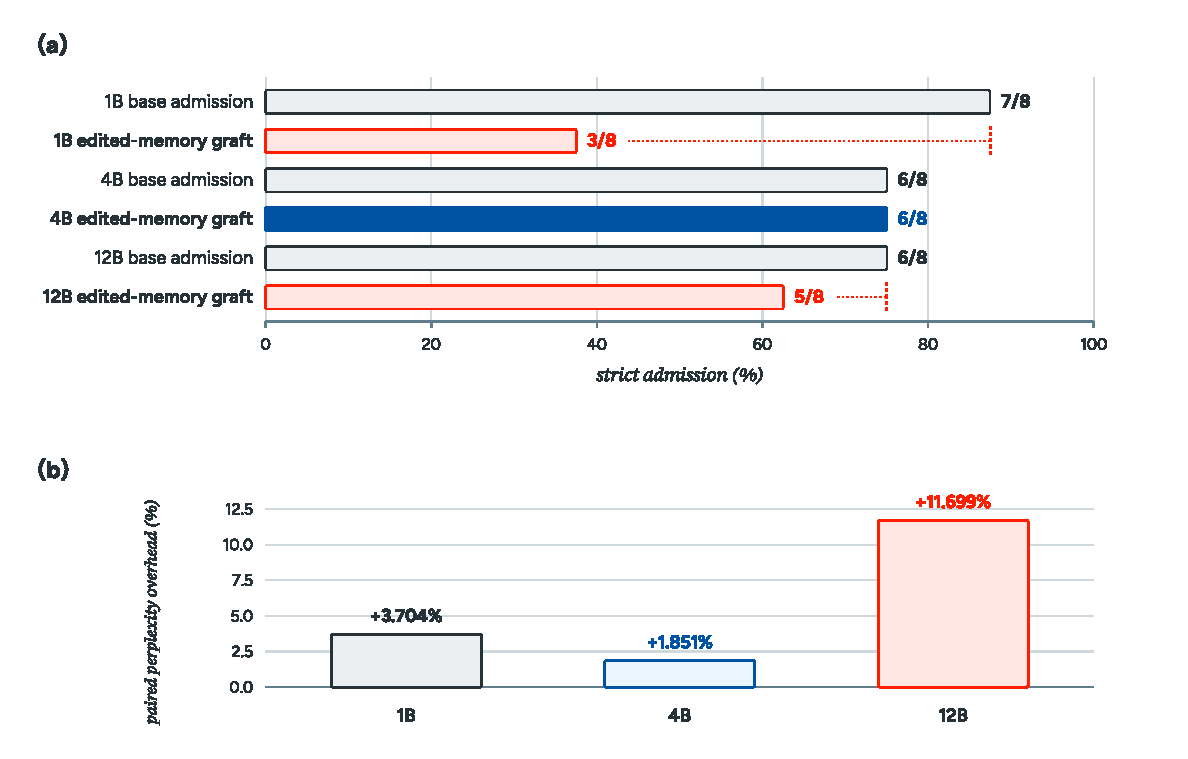
\includegraphics[alt={Across Gemma 1B, 4B, and 12B checkpoints, only 4B preserves base strict admission with low paired perplexity overhead.},width=\linewidth]{figs/audit_boundaries.pdf}
\caption{Admission and quality cost of the frozen configuration at three scales. (a)
Strict admission, where 4B is the only tested scale that preserves the base
model's eligibility. (b) Paired perplexity overhead, where 12B has the largest
measured quality cost. A dashed marker indicates that the graft no longer
matches its own base admission. The three checkpoints are sensitivity outcomes
and were not selected by any model-selection procedure.}
\label{fig:audit-boundaries}
\end{figure}

\FloatBarrier

We checked both agreement with the refit and completion of the decrement at
the two certified scales. At 1B, the median and maximum KL against the refit on retained keys are
\(1.86\times10^{-13}/1.25\times10^{-10}\); at 4B they are
\(2.36\times10^{-12}/6.48\times10^{-11}\). No probe exceeds \(10^{-6}\).
The reverse decrement failed its checks in \(396/640\) 1B and
\(2{,}020/3{,}040\) 4B attempted affected solves. Refitting completed each
of those updates, so every deletion still reached its reference. These
denominators include affected solves only; solve points before the deleted
position do not need an update. Scoring the already-constructed exact, refit, and decay states
takes 561.5 s for 32 probes at 1B and 2,354.6 s at 4B; these are the costs of
scoring the audit and do not measure deletion latency.

\subsection{Behavioral attack details}

At \(k=1\), exact-phrase leakage is \(0.28\%\) edited and \(0.42\%\)
never-stored. At \(k=200\), each condition leaks on \(3/18\) field queries
(\(16.7\%\), the cohort rate), with paired record-bootstrap difference
\(0.0\,[0.0,0.0]\). Present and prompt-only are \(18/18\) (\(100\%\)), and decay
is \(5/18\) (\(27.8\%\)). To check reproducibility, we repeated the sampling
arm with the same seeds, decoding settings, and batch size. It reproduced every
\(k=200\) endpoint exactly (\(18/18\), \(18/18\), \(3/18\), \(3/18\),
and \(5/18\) for present, prompt-only, edited, never stored, and decay) and
the \(k=1\) rates to within \(0.02\) percentage points, while individual
sampled completions differed. Thus the per-query endpoints reproduced on
this hardware even though the per-sample counts were not bit-exact.
Elicitation, related-data updates, and LiRA are described in the released
attack aggregate.

For LiRA AUC intervals, we resampled records with replacement and took
percentile endpoints over \(10^4\) draws: six-record
cohort \(0.534\) \([0.513, 0.601]\), broad cohort \(0.517\)
\([0.516, 0.539]\); AUCs computed separately for each record span \(0.47\)--\(0.76\) and
\(0.53\)--\(0.73\). The broad LiRA policy includes
\(16/512\) edited test deletions routed to raw repack. Replacing those scores
with arbitrary values moves the AUC anywhere in \([0.486,0.549]\); we report
that range as a sensitivity check, distinct from a confidence interval.
The frozen interval code sorts the 10,000 pooled AUCs and selects ordered
entries 251 and 9,750 (one-based), yielding the asymmetric broad interval
[0.5157394409179688, 0.5387916564941406]. It also reports the upper central
AUC computed separately for each record for even sample sizes. Table~\ref{tab:lira-results} keeps
these conventions and rounds only for display.

\section{LongMemEval protocols and complete counts}\label{app:longmemeval}

Section~\ref{sec:longmemeval} reports the findings of the two LongMemEval
studies. This appendix gives their protocols and the complete counts behind
each reported rate, beginning with the selected examples and then describing
the two cohorts.

\subsection{Selected decoded examples and their limits}\label{app:decoded-cases}

The mortgage, screwdriver, and tennis examples are post hoc illustrations
from the completed 96-history study, not additional experiments. Each target
has three nested suffix variants assembled from the pinned public LongMemEval
oracle, with the same target and retained control. The protocol deletes the
selected latest user--assistant round, preserves earlier evidence literally,
and leaves later retained turns unchanged. A fresh raw-history reference
re-encodes those retained inputs; it does not regenerate them. For each probe,
the model receives a registered user turn containing \texttt{Current Date:},
the official question, and ``Reply with only the remembered value, without
explanation.'' A model turn then begins. Repeated deterministic decodes are
reproducibility checks, not independent samples. Solver checks target the
fixed-$C$ problem on the retained keys; no separate refit response was decoded.

\paragraph{Mortgage update.}
The official target question is quoted in Section~\ref{sec:mortgage-case},
with query date December 9, 2023. The owned November 30 round occupies token
positions $[876,1233)$ in each assembled history. The earlier August 11 round
mentions pre-approval for \$350,000; the removed round mentions \$400,000.
The retained question, dated May 27, 2023, is ``I wanted to follow up on our
previous conversation about YouTube videos for workplace posture. Can you
remind me of the Mayo Clinic video you recommended?'' The saved benchmark gold
contains the video title ``How to Sit Properly at a Desk to Avoid Back Pain''
and URL \url{https://www.youtube.com/watch?v=UfOvNlX9Hh0}.

\begin{table}[ht]
\centering\small
\caption{All three mortgage variants. Entries are saved generated answers to
the target query; the video URL is present under all four conditions in every
variant. Variant 0's edited answer also includes the video title.}
\label{tab:mortgage-variants}
\begin{tabular}{@{}rrrrlll@{}}
\toprule
variant & tokens & after edit span & present & prompt & local edit & rebuild\\
\midrule
0 & 2,596 & 1,363 & \$400,000 & \$400,000 & \$350,000 & \$350,000\\
1 & 2,764 & 1,531 & \$400,000 & \$400,000 & \$350,000 & \$350,000\\
2 & 2,941 & 1,708 & \$400,000 & \$400,000 & \$350,000 & \$350,000\\
\bottomrule
\end{tabular}
\end{table}
The local policy used refit fallback in 480/560, 508/600, and 534/640 affected
head/solve-point solves, respectively. The high use of refitting leaves the speed advantage of a
local edit unestablished. The retained URL matches the broader endpoint in
all variants, although the registered whole-answer substring endpoint does
not match the complete gold sentence. Aggregate retained matching is
reported in Section~\ref{sec:mortgage-case}.

\paragraph{A local edit and rebuild can answer differently.}
For the screwdriver target, the earlier exchange says the small screwdriver
was misplaced. The latest user says ``I actually have a spare screwdriver'';
the assistant responds ``Spare screwdriver: Ah, excellent!'' [excerpts].
The deleted user--assistant round occupies $[1189,1594)$. The official query
is ``Do I have a spare screwdriver for opening up my laptop?''
Table~\ref{tab:screwdriver-variants} preserves the suffix-dependent outcome.
All conditions return ``38'' to an unrelated numerical control whose saved
gold is ``38 subjects''; neither existing retained matcher marks those answers
correct. The reported labels follow those registered matchers.

\begin{table}[ht]
\centering\small
\caption{All three screwdriver variants. Editing and rebuilding disagree in
variant 0; the other two rebuilt answers also contain the target ``Yes''.}
\label{tab:screwdriver-variants}
\begin{tabular}{@{}rrllll@{}}
\toprule
variant & tokens & present & prompt & local edit & rebuild\\
\midrule
0 & 3,160 & Yes & No & Yes & No\\
1 & 3,290 & Spare screwdriver & Yes & Yes & Yes\\
2 & 3,038 & Yes & No. & Yes & Yes\\
\bottomrule
\end{tabular}
\end{table}
The local policy used refit fallback in 538/600, 564/640, and 510/560 affected
solves. These examples show a difference in decoded behavior; they do not
identify which surviving row or later turn caused it.

\paragraph{A harder question can expose an endpoint limitation.}
The tennis target asks both previous and current frequency. Its full gold
answer says previously every week on Sunday and currently every other week
on Sunday. Across histories of 2,339, 2,356, and 2,674 tokens, present and
prompt-only conditions generate only ``Every other week'', whereas editing
and rebuilding generate ``Weekly''. The retained answer is
\texttt{MusicTheory.net} throughout. Neither partial target answer matches
the full registered gold, so matcher-negative output alone does not establish
successful forgetting. The frozen counts retain the registered matcher
labels for these incomplete answers.

The source question IDs are \texttt{852ce960} (mortgage),
\texttt{42ec0761} (screwdriver), and \texttt{f685340e} (tennis).
The source-free cohort manifest fixes all three history IDs and token spans
per target. The response audit connects the saved outputs to those histories,
and a local review manifest records their artifact paths and hashes.

\subsection{Bicycle and Speyer case: teacher-forced scores}\label{app:bicycle-case}

The bicycle example in the introduction comes from the 16-history pilot.
Its 3,103-token assembled history contains an earlier three-bike discussion;
the deleted round reports the new hybrid bike, updates the count to four,
and includes the assistant's echo. The retained exchange supplies the Speyer
phone number. We use teacher-forced scoring to see how deletion changes the
probabilities of the saved answers: the model receives each saved answer
token as it proceeds, and we record its probability. For ``How many bikes do I currently own?'',
the one-token gold ``4'' moves from rank 2 to rank 28 after editing.
The 22-token phone answer keeps rank 1 at its first token; its mean log
probability changes from $-2.31560\times10^{-5}$ to
$-4.64238\times10^{-5}$ nats per answer token. Because the previous gold
tokens are supplied during scoring, the phone-number result does not tell
us whether the model would generate the complete number on its own.
The maximum local output KL is $4.32788\times10^{-17}$ nats across two probes,
in the direction from the edited policy to the fixed-$C$ refit. The bicycle probe's distinct
KL from the raw rebuild to the edited policy is $0.00176439$ nats over the first-token vocabulary.
Of 560 affected solves, 522 used exact-refit fallback and 38 completed
incrementally. The record ID ends in \texttt{c8276e265e3db489c090cdcc}.

\LMChatMainResultText

\LMChatAppendixText



% POST-HOC DECODED FOLLOW-UP.
% Numerical claims are bound to:
%   gemma_sv/benchmarks/longmemeval_chat_v3_summary_v1.json
%   gemma_sv/benchmarks/longmemeval_chat_leakage_recall_census_summary_v2.json
%   gemma_sv/benchmarks/longmemeval_chat_leakage_recall_census_statistics_v3.json
%   gemma_sv/benchmarks/longmemeval_chat_human_validation_results_v1.json
%   gemma_sv/benchmarks/longmemeval_chat_leakage_recall_census_human_adjudicated_v4.json
% Full response text and private judge ledgers remain local-only.

\subsection{Decoded follow-up: cohort and decoding}\label{app:longmemeval-cohort}

The follow-up tests what the model actually generates on
\(K=\LMChatVThreeK\) target clusters and \(n=\LMChatVThreeN\) histories,
separate from the pilot above (Appendix Table~\ref{tab:cohort-denominators}).
We froze the \LMChatVThreeK{} clusters first and packed three histories per
cluster independently. Every history completed under four conditions: record
present, local deletion, rebuilding from the retained history, and a
prompt-only instruction to forget. This produced
\LMChatVThreePopulationN{} decoded outputs. We kept histories even when the
model failed to recall the record, so every rate below uses all
\LMChatVThreeN{} histories. Decoding each probe greedily twice produced
identical text and token identifiers, checking deterministic reproducibility
rather than variation across sampled answers.

\subsection{Screening for disclosure: a matcher, a judge, and two reviewers}\label{app:longmemeval-screening}

We screened the \LMChatVThreePopulationN{} decoded outputs in three stages.
First, a deterministic matcher compared each output with the source answer
under five checks applied together: a casefolded substring test, a test after
punctuation and articles are stripped, a numeric and unit test, a URL test,
and a named-entity test. An output that passed any of them counts as a
disclosure. There were \LMChatVThreeMatcherPositiveN{} of these, and we did
not review them further. Second, a language model judge
(GPT-5.6) read every one of the \LMChatVThreeMatcherCleanN{} outputs the
matcher had cleared, seeing the question, the reference answer, and the
candidate response but neither the condition nor the matcher's verdict, and
returned one of three labels: disclosure, no disclosure, or ambiguous. Every
request returned a valid response. Because the provider serves the judge
under a name that can change between calls, the local audit retains the
requested and returned model names along with the frozen prompt, response
schema, and every request and response.

Third, two reviewers read a sample of the outputs, blinded to condition.
The sample held the \LMChatVThreeHumanFlagN{}
outputs the judge had flagged and \LMChatVThreeHumanControlN{} outputs it had
cleared, the latter chosen by hash so that the choice could not depend on
their content (\LMChatVThreeHumanReviewN{} outputs in all). The first reviewer
labeled every output in the sample, and the second read the flagged outputs
the first had not labeled as disclosures (\LMChatVThreeHumanSecondaryTripleN{}
distinct texts) and agreed with the first on each. The
\LMChatVThreeHumanReviewN{} outputs contain only
\LMChatVThreeHumanUniqueTripleN{} distinct question, answer, and response
triples, because the same response text recurs across conditions. We count
outputs below, but the duplicate texts are not independent judgments.

Of the \LMChatVThreeHumanFlagN{} flagged outputs, the reviewers labeled
\LMChatVThreeHumanFlagLeakN{} as disclosures,
\LMChatVThreeHumanFlagNoLeakN{} as no disclosure, and
\LMChatVThreeHumanFlagAmbiguousN{} as ambiguous, and they labeled all
\LMChatVThreeHumanControlN{} controls as no disclosure. Every confirmed
disclosure was a form of the answer that the matcher had failed to recognize:
\LMChatVThreeHumanNormalizationN{} were normalization failures and
\LMChatVThreeHumanAliasMorphologyN{} were an alias or an inflected form of the
answer, and none was a paraphrase. Most reviewed outputs were selected
because the judge had flagged them. The review therefore characterizes those
flags and a control sample, rather than estimating how often each condition
discloses. The \LMChatVThreeJudgeAmbiguousN{} outputs the judge itself marked
ambiguous were not reviewed.

\subsection{Disclosure rates and the paired comparison}\label{app:longmemeval-rates}

For the endpoint an output counts as a disclosure when the matcher flagged it
or the reviewers labeled it one; for flagged outputs the reviewers did not
read, the judge's label stands. Ambiguous labels give a lower and an upper
count. The reviewed labels changed the aggregate counts as follows.
After review, the \LMChatVThreeMatcherCleanN{} outputs the matcher cleared hold
\LMChatVThreeEffectiveMatcherCleanLeakN{} disclosures, \LMChatVThreeEffectiveMatcherCleanNoLeakN{} non-disclosures, and
\LMChatVThreeEffectiveMatcherCleanAmbiguousN{} ambiguous outputs, against the
judge's \LMChatVThreeJudgeMissN{}, \LMChatVThreeJudgeNoLeakN{}, and
\LMChatVThreeJudgeAmbiguousN{} before review. Per history, the edited policy
disclosed the deleted answer in
\(\LMChatVThreePolicyLeakLowerN/\LMChatVThreeN\), the never-stored rebuild in
\(\LMChatVThreeRebuildLeakLowerN/\LMChatVThreeN\), the record-present run in
\LMChatVThreePresentLeakLowerN{}--\LMChatVThreePresentLeakUpperN{} of
\LMChatVThreeN{}, and the prompt-only instruction in
\LMChatVThreePromptLeakLowerN{}--\LMChatVThreePromptLeakUpperN{}. The paired
edited-minus-rebuild difference is
\(+\LMChatVThreeEditedMinusFreshLowerN/\LMChatVThreeN=+\LMChatVThreeEditedMinusFreshLowerPoints\)
percentage points, with a \(95\%\) interval of
\([\LMChatVThreeEditedMinusFreshLowerCILowerPoints,
\LMChatVThreeEditedMinusFreshLowerCIUpperPoints]\) (a bootstrap over the
\LMChatVThreeK{} clusters), and the prompt-minus-edited difference is at least
\LMChatVThreePromptMinusEditedLowerPoints{} points (interval
\([\LMChatVThreePromptMinusEditedLowerCILowerPoints,
\LMChatVThreePromptMinusEditedLowerCIUpperPoints]\)). These
intervals hold the labels fixed and do not include uncertainty from selecting
the control outputs or from the reviewers' judgments. The \(+2/96\)
difference does not resolve equivalence, because we set no equivalence margin
in advance. Against margins chosen afterwards, the upper end of the interval,
\LMChatVThreeEditedMinusFreshLowerCIUpperPoints{} points, misses a 5-point
margin and meets a 10-point one. The counts put the edit well below the
prompt instruction and within a few points of rebuilding on this probe,
with disclosures remaining under both procedures.

\subsection{Matching responses and correct responses}\label{app:longmemeval-correctness}

The edited policy returned exactly the same target response as the
never-stored rebuild in \LMChatVThreeTargetPolicyRebuildExactN{} of
\LMChatVThreeN{} histories, and the same response under at least one of the
matcher's normalizations in \LMChatVThreeTargetPolicyRebuildNormalizedN{}.
To assess retained memory, we also compared responses with their saved
answers. On the retained probe, the answer was correct under the matcher in
\(\LMChatVThreeRetainedPresentCorrectN/\LMChatVThreeN\) histories with the
record present, \(\LMChatVThreeRetainedRebuildCorrectN/\LMChatVThreeN\) after
the rebuild, and \(\LMChatVThreeRetainedPolicyCorrectN/\LMChatVThreeN\) under
the edited policy, and the edited policy's retained response matched the
record-present response under some normalization in
\(\LMChatVThreeRetainedPolicyPresentNormalizedN/\LMChatVThreeN\). This comparison matters because the edit and rebuild can agree on an
incorrect answer.

Two histories illustrate why response agreement and correctness need
separate measurements. We chose one from each suffix stratum by SHA-256 rank
before reading any response and kept every condition for each. In the history
whose suffix had no lexical contact with the deleted answer, the gold target
was ``38,'' but every condition answered ``37,'' including the record-present
control. The retained answer, ``Three,'' was stable throughout. Deletion
cannot uniquely explain a target error that was already present in the
control. In the history with lexical contact, the record-present and
prompt-only conditions answered ``5,'' while the rebuild and edit answered
``Four.'' Here the edit tracked the rebuild, but every condition missed the
paired retained restaurant. Both histories remain in the original cohort
and in the rates reported above.

\subsection{The frozen suffix}\label{app:longmemeval-suffix}

We examined the surviving suffix because later text can carry information
from a deleted exchange back into a rebuild. Copies can appear as an
assistant's echo, a derived value, or a summary; the delta-attention study
gives a worked example~\citep{kdaomission}. We scanned the turns after each
deleted record for lexical contact with the target answer and found it in
\LMChatVThreeSuffixContaminatedHistoryN{} of \LMChatVThreeN{} histories,
spanning \LMChatVThreeSuffixContaminatedClusterN{} of \LMChatVThreeK{}
clusters. The suffix was assembled from independent support sources and was
never generated downstream of the target, so contact marks possible
contamination and does not establish causal dependence. The scanner catches
explicit restatements and some normalized forms, generally misses derived
traces and summaries, and can match short or numeric strings. The detected count is neither a lower
nor an upper bound on contamination.

We assessed whether lexical contact was associated with the edited policy's residual
disclosures (the \LMChatVThreePolicyLeakLowerN{} of \LMChatVThreeN{} in
Section~\ref{sec:longmemeval}). Among the
\LMChatSuffixContactHistoryN{} histories with contact, \LMChatSuffixContactDisclosureN{} disclosed and
\LMChatSuffixContactNoDisclosureN{} did not; among the
\LMChatSuffixCleanHistoryN{} without contact, \LMChatSuffixCleanDisclosureN{}
disclosed and \LMChatSuffixCleanNoDisclosureN{} did not, for disclosure rates
of \(\LMChatSuffixContactRiskPct\%\) and \(\LMChatSuffixCleanRiskPct\%\)
(Fisher's exact test, two-sided, \(p=\LMChatSuffixFisherP\)). Disclosure was less frequent in the lexical-contact stratum. The
matcher missed \LMChatSuffixHumanConfirmedEditedMissN{} edited-policy output
that the judge then flagged, and the reviewers confirmed it, so the
cross-tabulation is unchanged from the judge's labels. Lexical contact
therefore does not explain the residual disclosure in this study. A broader
deletion request could also ask for later turns to be regenerated if they
were caused by the deleted record. Our frozen-history comparison does not
test that operation; it is discussed in the delta-attention
study~\citep{kdaomission}.

